 % The main file for CAMP reports
 % Don't put any content in here. 
 % Don't even include content files by using \input or \inlcude. 
 % Put your content to TEXT.TEX or include it there using \input.
 % Uses:
 %		SETTINGS.TEX	contains the settings for this document
 %		COMMANDS.TEX	contains commands which can be used while writing
 %		INFO.TEX			contains the author, title and so on for the cover
 %		COVER.TEX			formats the front cover of the document
 %		ABSTRACT.TEX	contains the abstract to be included (if needed)
 %		TEXT.TEX			contains the actual content of the document
 %		BIB.BIB				containt the BibTeX entries for the document
 
 
%% Draft document mode
%% Final document

\documentclass[headsepline,footsepline,11pt,a4paper,bibtotoc,listof=totoc,footexclude,oneside,BCOR12mm,DIV13]{scrbook}

%idxtotoc
%\documentclass[headsepline,footsepline,footinclude=false,oneside,fontsize=11pt,paper=a4,listof=totoc,bibliography=totoc]{scrbook}

\usepackage{graphicx}
\usepackage{caption}
\usepackage{subcaption}

\usepackage{amsmath}
\usepackage{amsthm}
\usepackage{listings}
\usepackage{tikz}
\usepackage{qtree}
\usepackage{pgfplots, pgfplotstable, filecontents}
\usepackage{algorithm,algorithmicx,algpseudocode}
\usepackage{booktabs}
\usepackage{placeins} % float barrier
\usepackage{flafter}  %  ensures that floats don't appear until after they appear in the code.
\pgfplotsset{compat=newest,width=13.5cm}

% include title and author information for the cover
% Set here the title, authors and other stuff to be used for the cover
% This file is used by MAIN.TEX

% set title, authors and stuff for the cover
\def\doctype{Master's Thesis in Informatics}
\def\title{Design and Prototypical Implementation of a High-Level Synchronization Component for Dynamic Updates of Task Run Queues in L4 Fiasco.OC/Genode}
\def\titleGer{Entwurf und Prototypische Implementierung einer High-Level Synchronisationskomponente fuer dynamische Updates von Task-Warteschlangen in L4 Fiasco.OC/Genode}
\def\author{Gurusiddesha Chandrasekhara}
\def\date{October 15, 2016}
\def\supervisor{Prof. Dr. Uwe Baumgarten}
\def\advisor{Daniel Krefft,M.Sc.; Sebastian Eckl,M.Sc.}
\def\getSubmissionDate{October 15, 2016}
\def\getSubmissionLocation{Munich}

% text to appear in the footer
\def\footertext{}


% include settings
\bibliography{bibliography/literature}{}

\setkomafont{disposition}{\normalfont\bfseries} % use serif font for headings
\linespread{1.05} % adjust line spread for mathpazo font

% Settings for glossaries TODO: remove the following block if glossary not needed
\renewcommand{\glsnamefont}[1]{\normalfont\bfseries #1} % use serif font for glossary entry titles
\makeglossaries{}

% Settings for pgfplots
\pgfplotsset{compat=1.9} % TODO: adjust to your installed version
\pgfplotsset{
  % For available color names, see http://www.latextemplates.com/svgnames-colors
  cycle list={CornflowerBlue\\Dandelion\\ForestGreen\\BrickRed\\},
}

% Settings for lstlistings
\lstset{%
  basicstyle=\ttfamily,
  columns=fullflexible,
  autogobble,
  keywordstyle=\bfseries\color{MediumBlue},
  stringstyle=\color{DarkGreen}
  }


% include commands
% Commands to be used within the TUM report document
% Included by MAIN.TEX
% Please include your own cool commands here. 
% Be only sure to comment it sufficiently so others can use it.

%-------------------------------------------------------------
%                      Own Commands
%-------------------------------------------------------------
\DeclareMathOperator*{\st}{\text{ s.t. }}
\DeclareMathOperator*{\rev}{rev}
\DeclareMathOperator*{\enc}{enc}
\DeclareMathOperator*{\argmin}{argmin}
\DeclareMathOperator*{\argmax}{argmax}

\DeclareMathOperator*{\prerank}{pre-rank}
\DeclareMathOperator*{\postrank}{post-rank}

\DeclareMathOperator*{\preselect}{pre-select}
\DeclareMathOperator*{\postselect}{post-select}

\DeclareMathOperator*{\firstchild}{first-child}
\DeclareMathOperator*{\lastchild}{last-child}
 
\DeclareMathOperator*{\nextsibling}{next-sibling}
\DeclareMathOperator*{\prevsibling}{prev-sibling}

\DeclareMathOperator*{\nextsiblingk}{next-sibling^{k-1}}
\DeclareMathOperator*{\prevsiblingk}{prev-sibling^{k-1}}
\DeclareMathOperator*{\enclosek}{enclose^{d}}

\DeclareMathOperator*{\subtreesize}{subtree-size}

\DeclareMathOperator*{\fwdsearch}{fwd-search}
\DeclareMathOperator*{\bwdsearch}{bwd-search}

\DeclareMathOperator*{\parent}{parent}
\DeclareMathOperator*{\enclose}{enclose}
\DeclareMathOperator*{\rmqi}{rmqi}
\DeclareMathOperator*{\rmq}{rmq}
\DeclareMathOperator*{\RMQ}{RMQ}
\DeclareMathOperator*{\RMQi}{RMQi}
\DeclareMathOperator*{\findopen}{findopen}
\DeclareMathOperator*{\findclose}{findclose}
\DeclareMathOperator*{\inspect}{inspect}
\DeclareMathOperator*{\isleaf}{isleaf}
\DeclareMathOperator*{\isancestor}{isancestor}
\DeclareMathOperator*{\depth}{depth}
\DeclareMathOperator*{\levelnext}{level-next}
\DeclareMathOperator*{\levelprev}{level-prev}
\DeclareMathOperator*{\levellmost}{level-lmost}
\DeclareMathOperator*{\levelrmost}{level-rmost}
\DeclareMathOperator*{\deepestnode}{deepest-node}
\DeclareMathOperator*{\levelancestor}{level-ancestor}
\DeclareMathOperator*{\lca}{lca}
\DeclareMathOperator*{\ssum}{sum}
\DeclareMathOperator*{\childselectfromleft}{left-select-child}
\DeclareMathOperator*{\childselectfromright}{right-select-child}

\DeclareMathOperator*{\rankopen}{rank_1}
\DeclareMathOperator*{\rankclose}{rank_0}

\DeclareMathOperator*{\selectopen}{select_1}
\DeclareMathOperator*{\selectclose}{select_0}

\DeclareMathOperator*{\selectopenfrom}{selectfrom_1}
\DeclareMathOperator*{\selectclosefrom}{selectfrom_0}

\DeclareMathOperator*{\excess}{pi}
\DeclareMathOperator*{\opencounter}{phi}
\DeclareMathOperator*{\closecounter}{psi} 

%-------------------------------------------------------------
% math stuff -------------------------------------------------

% nice R, N, C
\newcommand{\nat}{\mathbb{N}}
\newcommand{\real}{\mathbb{R}}
\newcommand{\compl}{\mathbb{C}}

% norm
\newcommand{\norm}[1]{\left\| #1 \right\|}

% un demi
\newcommand{\half}{\frac{1}{2}}

% parantheses
\newcommand{\parenth}[1]{ \left( #1 \right) }
\newcommand{\bracket}[1]{ \left[ #1 \right] }
\newcommand{\accolade}[1]{ \left\{ #1 \right\} }
%\newcommand{\angle}[1]{ \left\langle  #1 \right\rangle }

% partial derivative: %#1 function, #2 which variable
% simple / single line version
\newcommand{\pardevS}[2]{ \delta_{#1} f(#2) }
% fraction version
\newcommand{\pardevF}[2]{ \frac{\partial #1}{\partial #2} }

% render vectors: 3 and 4 dimensional
\newcommand{\veciii}[3]{\left[ \begin{array}[h]{c} #1 \\ #2 \\ #3	\end{array} \right]}
\newcommand{\veciv}[4]{\left[ \begin{array}[h]{c} #1 \\ #2 \\ #3 \\ #4	\end{array} \right]}

% render matrices: 3  dimensional (arguments in row first order)
\newcommand{\matiii}[9]{\left[ \begin{array}[h]{ccc} #1 & #2 & #3 \\ #4 & #5 & #6 \\ #7 & #8 & #9	\end{array} \right]}
%DOESN'T WORK,DON'T KNOW WHY \newcommand{\mativ}[16]{\left[ \begin{array}[h]{cccc} #1 & #2 & #3 & #4 \\ #5 & #6 & #7 & #8 \\ #9 & #10 & #11 & #12 \\ #13 & #14 & #15 & #16 \end{array} \right]}


%-------------------------------------------------------------
%-------------------------------------------------------------


%-------------------------------------------------------------
% some abreviations ------------------------------------------
\newcommand{\Reg}{$^{\textregistered}$}
\newcommand{\reg}{$^{\textregistered}$ }
\newcommand{\Tm}{\texttrademark}
\newcommand{\tm}{\texttrademark~}
\newcommand {\bsl} {$\backslash$}

%-------------------------------------------------------------
%-------------------------------------------------------------


%-------------------------------------------------------------
% formating --------------------------------------------------

% Theorem & Co environments and counters
\newtheorem{theorem}{Theorem}[chapter]
\newtheorem{lemma}[theorem]{Lemma}
\newtheorem{corollary}[theorem]{Corollary}
\newtheorem{remark}[theorem]{Remark}
\newtheorem{definition}[theorem]{Definition}
\newtheorem{equat}[theorem]{Equation}
\newtheorem{example}[theorem]{Example}
%\newtheorem{algorithm}[theorem]{Algorithm}

% inserting figures
\newcommand{\insertfigure}[4]{ % Filename, Caption, Label, Width percent of textwidth
	\begin{figure}[htbp]
		\begin{center}
			\includegraphics[width=#4\textwidth]{#1}
		\end{center}
		\vspace{-0.4cm}
		\caption{#2}
		\label{#3}
	\end{figure}
}




% referecing figures

\newcommand{\refFigure}[1]{ %label
	figure \ref{#1}
}
\newcommand{\refChapter}[1]{ %label
	chapter \ref{#1}
}

\newcommand{\refSection}[1]{ %label
	section \ref{#1}
}

\newcommand{\refParagraph}[1]{ %label
	paragraph \ref{#1}
}

\newcommand{\refEquation}[1]{ %label
	equation \ref{#1}
}

\newcommand{\refTable}[1]{ %label
	table \ref{#1}
}




\newcommand{\rigidTransform}[2]
{
	${}^{#2}\!\mathbf{H}_{#1}$
}

%code, in typewriter
\newcommand{\code}[1]
 {\texttt{#1}}

% comment that appears on the border - very practical !!!
\newcommand{\comment}[1]{\marginpar{\raggedright \noindent \footnotesize {\sl #1} }}

% page clearing
\newcommand{\clearemptydoublepage}{%
  \ifthenelse{\boolean{@twoside}}{\newpage{\pagestyle{empty}\cleardoublepage}}%
  {\clearpage}}


%-------------------------------------------------------------
%-------------------------------------------------------------


\newcommand{\etAl}{\emph{et al.}\mbox{ }}


\makeglossary

\begin{document}

\frontmatter
	
\begin{titlepage}
  % HACK for two-sided documents: ignore binding correction for cover page.
  % Adapted from Markus Kohm's KOMA-Script titlepage=firstiscover handling.
  % See http://mirrors.ctan.org/macros/latex/contrib/koma-script/scrkernel-title.dtx,
  % \maketitle macro.
  \oddsidemargin=\evensidemargin\relax
  \textwidth=\dimexpr\paperwidth-2\evensidemargin-2in\relax
  \hsize=\textwidth\relax

  \centering

  \vspace{40mm}
  
\includegraphics[width=40mm]{logos/tum}

  \vspace{5mm}
  {\huge\MakeUppercase{\getFaculty{}}}\\

  \vspace{5mm}
  {\large\MakeUppercase{\getUniversity{}}}\\

  \vspace{20mm}
  {\Large \getDoctype{}}

  \vspace{15mm}
  {\huge\bfseries \getTitle{}}

  \vspace{15mm}
  {\LARGE \getAuthor{}}

  \vspace{20mm}
  
\includegraphics[width=20mm]{logos/faculty}
\end{titlepage}


\clearemptydoublepage
	
% The titlepage for the CAMP report document.
% Included by MAIN.TEX


%--------------------------------------------------
% The title page
%--------------------------------------------------

% correct BCOR - undo at the end !!!
\def\bcorcor{0.15cm}
\addtolength{\hoffset}{\bcorcor}

\thispagestyle{empty}

 \vspace{10mm}
\begin{center}
	       \oTUM{4cm}
	   
	   \vspace{5mm}     
	   \huge FAKULT{\"A}T F{\"U}R INFORMATIK\\ 
	   \vspace{0.5cm}
	 \large DER TECHNISCHEN UNIVERSIT{\"A}T M{\"U}NCHEN\\
        
	\end{center}
		

\vspace{10mm}
\begin{center}

   {\Large \doctype}

  \vspace{10mm}
  
  {\LARGE \title}\\
  
  
  \vspace{10mm}
  
  
  {\LARGE  \titleGer}\\
  
  
  \vspace{10mm}

    %\hfill
    \begin{tabular}{ll}
	   \Large Author:     & \Large \author \\[2mm]
	   \Large Supervisor:    & \Large \supervisor \\[2mm]				
	   \Large Advisors:	& \Large \advisor\\[2mm]
	   \Large Date:       & \Large \getSubmissionDate
	 \end{tabular}
	 
	 \vspace{5mm}
	 
	 \begin{figure}[h!]
  \centering
   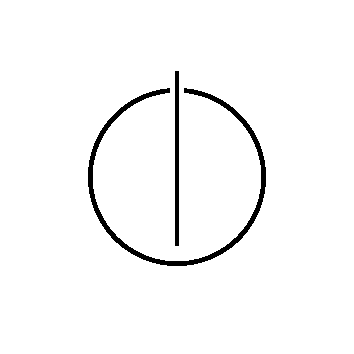
\includegraphics[width=4cm]{styles/informat.png}
  \end{figure}
   

\end{center}

% undo BCOR correction
\addtolength{\hoffset}{\bcorcor}

	
\thispagestyle{empty}
\vspace*{0.8\textheight}
\noindent
I confirm that this \MakeLowercase{\getDoctype{}} is my own work and I have documented all sources and material used.

\vspace{15mm}
\noindent
\getSubmissionLocation{}, \getSubmissionDate{} \hspace{5cm} \getAuthor{}

\cleardoublepage{}

 
\addcontentsline{toc}{chapter}{Acknowledgments}
\thispagestyle{empty}

\vspace*{20mm}

\begin{center}
{\usekomafont{section} Acknowledgments}
\end{center}

\vspace{10mm}

%TODO: Acknowledgments

%Writing this master's thesis would not have been possible without the help of these people. 
%First, I would like to thank my advisors Daniel Krefft and Sebastian Ekcl, who immediately accepted my request to do masters thesis and guided me to chose the projects. Special thanks to Daniel Krefft for his brilliant advices which he has given me every time we had a discussion.
%
%Thanks to Prof.Baumgarten for allowing me to do my research and for providing all the facilities at the chair. 
%
%Thanks to Paul Nieleck, who is finished his master thesis at the department for excellent collaboration and sharing his knowledge on the project. 
%
%Thanks to Alexander Reisner who is working at the department, for sharing his timely invaluable experience on the project. 
%
%%Thanks to Madhura Kumaraswamy for her help during my thesis. 
%
%Thank you to my family for providing me the freedom and support that required me to come to Germany for doing my masters. 


\cleardoublepage{}

	
\chapter{\abstractname}

%TODO: Abstract

%Motivation/Problem statement Aims and objectives

This thesis introduces a method for updating the task ready queues in the Genode Operating System Framework and the L4/Fiasco.OC microkernel. The presented method will be used in Organic Computing paradigm's Observer-Controller architecture. The Observer monitors the system and gathers the data and passes it to the Controller, which processes the data and takes a decision to schedule the tasks. This requires a method in place to provide the synchronized access to ready queue and update the tasks.

%What does the thesis do?
%The limitations in accessing the kernel ready queue from a high-level component led to the development of a split module. Accordingly,
The implementation of the ready queue update mechanism consists of a high-level Genode component and a low-level kernel module. The Genode component communicates with the Controller via a shared dataspace and receives the tasks to be updated and then passes them to the kernel module. The kernel module identifies the corresponding kernel threads and updates them to the ready queue. Various synchronization methods are presented in this thesis with special importance to lock-free algorithms. RCU and STM synchronization methods are suggested for synchronizing the kernel ready queue access. 

%Findings and conclusions
Tests of the task-ready queue update mechanism showed that the threads can be updated successfully to the ready queue and executed. On the other hand, complete ready queue swapping leaves the system in an unstable state. The high-level component is able to communicate successfully with the Controller via Genode's shared dataspace. The proposed design and implementation can be successfully used in the Observer-Controller architecture and it serves as a good starting point for the KIA4SM project's goal of having the ready queue update mechanism as a fully high-level component.

%vision of providing a homogeneous execution environment for heterogeneous hardware systems involves in using universally applicable ECUs and having flexible task scheduling on ECUs. This requires having a intelligent system in place to take decisions, which is solved by Organic-Computing paradigm's Observer-Controller architecture, which has an Observer that monitors the system and gathers the data and pass it to the Controller, which processes the data and takes a decision to schedule the tasks. This requires a method in place to provide the synchronized access to ready queue and update the tasks.

\tableofcontents
  
\mainmatter
	
	
\chapter{Introduction}
The implemented high-level synchronization component in this master thesis is part of the KIA4SM project of the department of operating systems. The work aims to implement a method for dynamic update of tasks ready queues in L4 Fiasco.OC/Genode while providing a synchronized access to them.



  

\section{Overview of KIA4SM project}

KIA4SM (stands for Cooperative Integration Architecture for Future Smart Mobility Solutions) is a research project at the department of operating systems. Traditionally Cooperative Intelligent Transport Systems have been built on heterogeneous systems. KIA4SM aims to provide an architecture of having an homogeneous platform for heterogeneous systems. 

KIA4SM focuses on developing systems for the interaction and coordination between computer-assisted vehicles, be it partially or fully autonomously functioning actors.  KIA4SM aims to improve on the ad-hoc networking between vehicles

The final vision of the project is illustrate in (Fig). The goals of the project are,

\begin{itemize}
\item A common platform as foundation for device in-
dependent (vehicles, mobile devices, traffic and
transport architecture) provision and execution of
software-based functionality
\item Mechanisms that allow for online dynamic reconfig-
uration, based on
\begin{itemize}
\item en-/disabling and relocation/migration of
software-based functionality
\item adaptive (data-centric) routing policy
\item flexible scheduling of tasks per ECU
\end{itemize}
\end{itemize}

In order to achieve the goals of the project a number of different methods have been applied. This has led to the application of Organic computing paradigm. igner and user.
Organic Computing (OC) has the vision to address the
challenges of complex distributed systems by making them more
life-like (organic), i.e. endowing them with abilities such as self-
organization, self-configuration, self-repair, or adaptation.
%Refer: paper: Organic Computing – Addressing Complexity by Controlled Self-organization 
In order to realize this, universally applicable Electronic Control Units (ECU) and a common run-time environment are used which provides Hardware/Software Plug-and-Play properties.

\section{Motivation}

There are number of micro controllers used for different calculations in a modern vehicle, this project aims to replace them with use more power-full and standardized hardware universally applicable ECUs. 

OC approach proposes a Observer-Controller architecture similar to MAPE architecture(monitor, analyze, plan, execute) . An observer collects the data from the all the ECUs and computes and generates indicators where a controller takes a decision based on the indicator, generates an action.

One such action of the controller is to decide what tasks should be executed at what time in order to meet the aforementioned requirements of the safety critical systems. So the controller decides and produces a run/ready queue (RQ). There needs to be a method which allows to safely update the scheduler run queues of the system. 

Therefore it is essential to be able to add threads and modify the execution order 
during operation time, A flexible thread handling is also required for example in case 
a ECU is malfunctioning. In this case it would be possible to swap the threads from the 
malfunctioning one to working ones. So it is important to generate new ready-queues 
based on the information we are receiving from the other ECUs in the grid, and then 
exchange them with the actual ready-queue the scheduler uses.

\section{Thesis structure}
The thesis is structured in a way that the reader understands the importance of the work carried out here and also the surrounding concepts before delving in to the specifics (inverted traingle). 

The second chapter summarizes the related work on the state of the art algorithms for synchronization and different types of schedulers in use and at the end of the section an evaluation of the synchronization methods is provided inorder to chose the best possible approach for the existing project.

The third chapter explains the Genode and L4 Fiasco.OC details in brief, in order for the user to have an overview of the system. 

The fourth chapter deals with the design considerations along with implementation details.

The fifth chapter is dedicated to explains testing method and the results obtained.
And the final chapter concludes the thesis with the limitations and future work to be done. 

\chapter{Related Work}
This chapter explains the previous work and concepts which led to the development of synchronization component to the KIA4SM project. 
It explains the synchronization algorithms available and makes a comparative study of these algorithms. 
The comparative study is based on the research work of many papers which are referred here. An attempt is made to pick the best choice algorithm for the work. 

\section{Synchronization of L4 fiasco tasks}

The thesis is largely based on the work of Robert H{\"a}cker, who in his bachelor thesis \textit{ "Design of an OC-based Method for efficient Synchronization of L4 Fiasco.OC Mircrokernel Tasks"} \cite{haecker}, explains the design of a scheduler best suited scheduler for KIA4SM project and also gives comparison study of the different schedulers and synchronization methods suited for updating the task ready queue. 

He suggests Modified-Maximum-Urgency-First algorithm as the best choice for KIA4SM project due to the importance of safety and security in embedded systems. After comparing the synchronization algorithms the sequential lock technique has been chosen for the better control it gives. He has suggested to verify the practical implication of Read-Copy Update(RCU). At the end he proposes a design for the existing system including aforementioned  scheduler(MMUF) and sequential locks. 

This work is an extension of H{\"a}cker's findings. However, the focus of the thesis it to develop a good synchronization method, the implementation of the scheduler is not carried out. As go forward I make reference to Robert H{\"a}cker's work. 

Some of the ideas and code knowledge is taken from the Valentin Hauner's bachelor's thesis \textit{"Extension of the Fiasco.OC microkernel with context-sensitive
scheduling abilities for safety-critical applications in embedded systems"} \cite{hauner}. In this thesis he added EDF scheduling strategy. Though his thesis concentrated on using it in Genode and L4RE environment, it helped in understanding the scheduler.

\section{Synchronization Methods}

To do the justification to many synchronization methods are studied and are explained in this section. The synchronization categories are divided based on the methods they apply. 
The figure %TODO insert the picture 
shows the different types of synchronization methods along with examples. 

\subsection{Lock-based algorithms}

\subsection{Lock-Free algorithms}

\chapter{ Genode OS framework and L4 Fiasco.OC}

\section{section}

I cite \cite{Navarro_Sadakane}

\chapter{Design and Implementation}
\chapter{Testing and Results}
\chapter{Conclusion}

\section{Limitations}
\section{Future Work}


		
		
		
		% ---------------------------------------------------------------------------
		%
		% Appendix
		%
		% ---------------------------------------------------------------------------
		
%		\part*{Appendix}
%		\addcontentsline{toc}{part}{Appendix}
		
%		\appendix %---------------------------------------
		
%		\input{chapters/oneAppendix}
		
	


  \clearemptydoublepage
	\bibliography{bibliography/bibliography}
	
	\listoffigures
	\listoftables 
 
\end{document}

